\chapter{Implemention}
	\section{How the program works}
	This section describes how to set up the prototype, connect the camera, limitations of the program and all that jazz.
	\subsection{VR}
	Something about VR toolkit in Unity
	\section{DLLs and Unity}
		When discussing the initial idea at the semester workshop it was suggested that we implement the design in the Unity game engine\footnote{Unity's homepage \url{https://unity3d.com/}}, as it allows for high-level management of objects in space, and would reduce development time on the part of the implementation not concerned with image processing. Unity has a fair number of different options for performing image processing. However, as we would be creating the fiducial markers from scratch we could not use any preexisting software. We were already familiar with openCV, a fast library for image processing and computer vision, so developing using openCV made sense.\\\\
		One issue is that Unity uses C\# and openCV is only developed for C++, C, Python, and Java. The method used in this project to bridge this language barrier is to compile the C++ code as a DLL, or "Dynamic Linked Library", and import it into the C\# code. DLLs  cannot be executed in the way normal applications are, and are instead designed to be used by other applications. Because they can be complied from a host of different languages they are not limited to what C\# code can do. Another advantage is that they are compiled in machine code and are therefore very fast\footnote{How to Write Native Plugins For Unity \url{https://www.alanzucconi.com/2015/10/11/how-to-write-native-plugins-for-unity/}}. However, there are a number of disadvantages with this implementation that must be taken into consideration, and which have made the process of completing this project less smooth. As Unity and the plug-in do not have access to each other's code, passing an object between the two is difficult, for example. For the same reason, debugging crashes is tricky. During development of this project, one fatal bug consistently crashing the program happened in an unmanaged part of Unity, so Unity could not give an error message. The code was developed in C++ which had no console where a log could be printed. Therefore troubleshooting became the source of a lot of frustration.\\\\
		Importing a function into DLL is simple, as seen in Listing \ref{listing:dllExport}.
\begin{listing}[H]
\caption{How to: declare a function for DLL export}
\label{listing:dllExport}
\begin{minted}[frame=lines, framesep=2mm,baselinestretch=1.1,fontsize=\footnotesize,linenos]{cpp}
extern "C" __declspec( dllexport ) int MyFunc(long parm1);
\end{minted}
\end{listing}
\codeword{extern "C"} tells the compiler that the function name should not be changed when it is compiled, so that its name is known when it is being imported into Unity. \codeword{__declspec()} tells the linker to do something. In this case \codeword{dllexport}, which tells it that it should export a function to a DLL. Therefore \codeword{__declspec(dllimport)} will be used to import the function in Unity. A sample call might look like this\\
\begin{listing}[H]
	\caption{How to: declare a function for DLL import}
	\label{listing:dllImport}
	\begin{minted}[frame=lines,
	framesep=2mm,baselinestretch=1.1,fontsize=\footnotesize,linenos]{cpp}
[DllImport("unityOpencvPlugin", EntryPoint = "init")]
public static extern int Init(ref int outCameraWidth, ref int outCameraHeight);
	\end{minted}
\end{listing}
The name of the DLL file "unityOpencvPlugin" is given as the "entrypoint". Unity will then do a search for a function called \codeword{init} in the DLL "unityOpencvPlugin". It is important that the function name is not changed when exporting, or this process will fail. In line 2; a function is declared that will call the imported function. It is important to note that this function must have the same signature (return type and arguments). Unity cannot check whether or not this is true, so it will proceed as if it is the case. Signature compatibility is sensible and straightforward for primitive types like \codeword{int}, but for objects it becomes a bit more tricky. It requires the declaration of similar objects in both languages, with variables in the same order. Otherwise the data will not make sense when returned. As an example, we need to return the markers found after image processing. They are represented in a structure: 
\begin{listing}[H]
	\caption{Objects in C\# and C++}
	\label{listing:objects}
	\begin{minted}[frame=lines, framesep=2mm,baselinestretch=1.1,fontsize=\footnotesize,linenos]{c++}
			//in C++
struct ObjectData{
ObjectData(int x, int y, int type, int color) : X(x), Y(y), Type(type), Color(color) {}
int X, Y, Type, Color;
};
			//in C#	
[StructLayout(LayoutKind.Sequential, Size = 16)]
public struct CVObject{
public int X, Y, Type, Color;
}
	\end{minted}
\end{listing}
In Unity the structure needs to be laid out sequentially when exported to unmanaged memory.\footnote{Unity layout \url{https://msdn.microsoft.com/en-us/library/system.runtime.interopservices.layoutkind(v=vs.110).aspx}}. In order to detect several objects it is easier to pass a pointer to an array, and make C++ fill it out from the code. A few things are needed for this to work. The function needs to take a pointer as an argument, and the size of the array must be passed as an argument, so that the method does not overwrite data outside of the array. The memory that the pointer points to must not remain static, or the pointer would no longer point to the right data. In C\# the keyword \codeword{Fixed} prevents data from being moved in memory, and \codeword{unsafe} enables working with pointers. Below is an example from our implementation in the project where we pass a pointer to C++. %be careful with "unsafe" though. It oftentimes leads to children. 
\begin{listing}[H]
\caption{The function call to pass a pointer to C++, which is filled by the code}
\label{listing:pointer}
\begin{minted}[frame=lines,
		framesep=2mm,baselinestretch=1.1,fontsize=\footnotesize,linenos]{c++}
unsafe{
	fixed (CVObject* outMarkers = _markers){
		Cap(outMarkers, _maxMarkerDetectCount, ref detectedMarkersCount);
	}
}
\end{minted}
\end{listing}

\section{BGR to RG chromaticity conversion}
Its was found that differences in lighting conditions made thresholding the feed from the camera at best suboptimal. To circumvent this the feed is converted to rg chromaticity, also known as normalized rgb, and henceforth RG. RG contains no intensity information and as such is not a color space but instead a chromatic space\footnote{\url{https://en.wikipedia.org/wiki/Chromaticity}}.
\subsection{Theory of RG} \todo{maybe move to analysis}
The critical property that RG has is it does not record the individual channels intensity, but rather the color's intensity as a percentage of the total intensity. Mathematically the RG value of a channel can be derived from an RGB value in the following way.
\[ RG_x = \frac{RGB_x}{RGB_1 + RGB_2 + RGB_3}\]
where x represents which of the channels that is to be converted. This will give a value between 0 and 1 depending on how big a percentage of the total intensity comes from that color. However, since floats are operationally slow it is advised to scale the value to 8bits by multiplying by 255. If one where to convert all three, with capital letter representing the RG chromaticity, the channels can be found as.
\[ RED = \frac{red}{red + blue + green} * 255\]
\[ BLUE = \frac{blue}{red + blue + green} * 255\]
\[ GREEN = \frac{green}{red + blue + green} * 255\]
This means that in RG the sum of all channels must be 255.
\[ \frac{red}{red + green + blue} + \frac{green}{red + green + blue} \frac{blue}{red + green + blue} =  \frac{red + green + blue}{red + green + blue} = 1\]
It is observed that in RG the channel values are codependent. If the value of red is large, then the other channels must by definition contain small value as they all must add up to 255. A result of this is that one can find the value in one channel if the other two are known.
\[ BLUE = 255 - RED - GREEN\]
So it is possible to store the data using two bits, and calculate the third color if it is needed. This loss of information comes from the loss of intensity data\cite{NormRGB}. for example two colors (0,10,50) and (0,50,250) will produce exactly similar value when converted to RG. 
\[ BLUE = \frac{50}{50 + 10} * 255 = (int)212.5 = 212 \]
\[ BLUE = \frac{250}{250 + 50} * 255 = (int)212.5 = 212 \]
The same is true for any two color that are proportionately similar.\\
\todo{creat image showing (0,10,50) and the other, after conversion to (0,42,212)} 
In relation to image processing one has to be aware that noise, particularly in shadows, mess with the rg space. For this reason it is recommended to zero the values if the total sum is below a certain value.

\subsection{Thresholding in RG}
\todo{write a bit more about the implication of each threshold}
Because RG can be represented by two values it is possible to plot the  chromaticity space using two axes, as can be seen in figure \ref{fig:rgbNorm}
\begin{figure}[H]
	\centering
	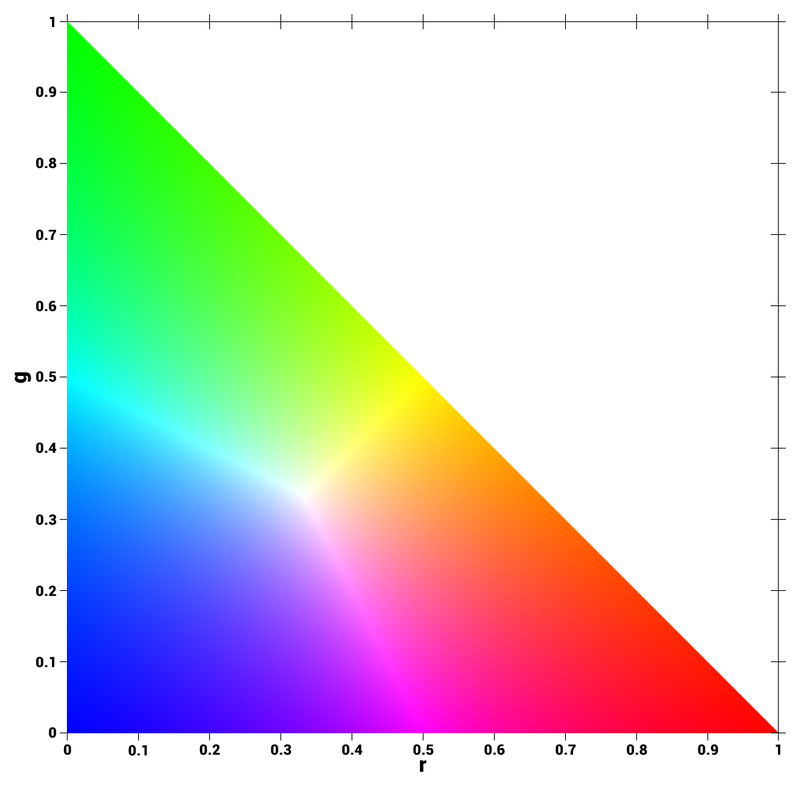
\includegraphics[width=0.5\linewidth]{figure/Analysis/normRGB.png}
	\caption{The entire RG color space is visible here, it can be represented in 2D due to the loss of intensity data that happens during conversion.}
	\label{fig:rgbNorm}
\end{figure}
There are different ways to threshold in RG, and because of the two dimensionality they are wonderfully reminiscent of high school math. Common amongst all of the presented values is that they use the red and green values of each pixel to determine whether the pixel should be set to 255
 or 0.\\
\textbf{In range}, is an often used way of thresholdnig in the HSV color space\footnote{\url{https://docs.opencv.org/3.2.0/df/d9d/tutorial\_py\_colorspaces.html}}. One sets a range in each axis in which to threshold. For example between 160 to 255 in red, and 0 to 60 in green. The thresholding consists of comparing the red and green value in each pixel to the ranges. If both values are inside the designated range the pixel is set to 255, else it is set to 0. This will create a square segmentation in the chromaticity space. It should not surprise anyone because we are comparing two constants. Constants create straight lines. \todo{create img}\\

\textbf{Line threshold}. Is another potential way to threshold. One creates a straight line with a formula $ y = ax - b$. Where y and x each represent the two axes. $a$ decides the slope of the line and is controlled by $x$ which is one of the color. In this case, lets say $x$ is red. $b$ decides where the thresholding should start and can be found using $b =- i * a$. Where $i$ is the start point of the line. Based on the equation we can find value of green that would place it on the line for a given red value. Then our values can be compared the line to see which side of the line it is on. If the values are on the right side it to 255, else set it to zero.\\

\textbf{Distance threshold}. Is based on finding the chromaticity distance from the a pixels color to a reference value in RG. If the distance is below a threshold the set it to 255, else 0. In two dimensions the distance between two points, $p_0$ and $p_1$, can be found as $d = \sqrt{(p_1x - p_0x)^2 +(p_1y - p_0y)^2}$. In our implementation we used a red value of 180 and a green value of 40 for our reference color. The threshold distance was set to 60. This produces a the following threshold.\\
In the end we decided to implement a distance based threshold because it allows for more lighting change resistant thresholding of the color red. Now that the reasons for our choices have been laid out, we might as well move into how these actually were implemented into our code.
\subsection{rg chomaticity in code}
The process of converting an rgb image described above is a matter of simple point processing. We have made a few changes to speed up the process at runtime. The current code performs these two steps at each pixel in the input image.\\
\begin{enumerate}
	\item Find the sum of the rgb chanels.
	\item Assign the corresponding pixel in the output to the value found in a look up table using the sum and value in the channel\\
\end{enumerate}
Really the only big change is the decision to use a look up table. A look up table is useful if you are going to be performing the same operation on similar data a lot of times. 
\subsection{Creating a lookup tabel}
The concept of a lookup table is, "instead of calculating this thing every time, why don't i calculate a table with the results of all possible inputs and just look up what the result is". This might sound like madness until one realizes the magnitude of data we are working with. The webcam that we use has a resolution of 640 x 480. That is 307200 pixel. Now mulitplications and additions are very fast and generally faster than memory access\todo{references for this}. Division is a more expensive operation and we have to do division and multiplication three times per pixel (one for each channel). We found that at runtime using a look up table increased the speed of our conversion algorithm by 100.25\% as can be seen in listing \ref{rgConvSpeed}. 
\begin{center}
	\begin{multicols}{2}


	\begin{multicols}{2}
		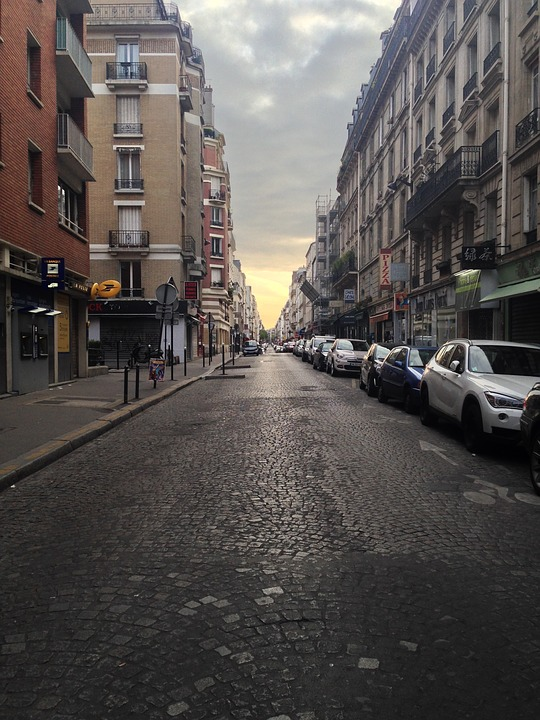
\includegraphics[width=1\linewidth]{figure/Analysis/city.jpg}
	  \columnbreak
		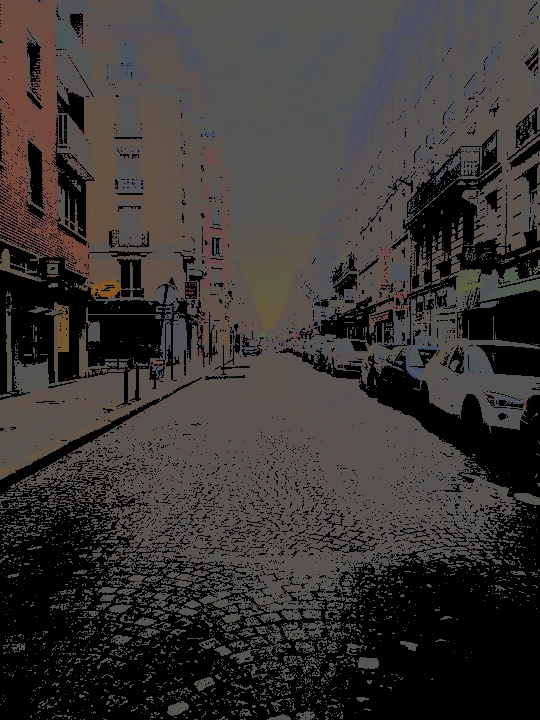
\includegraphics[width=1\linewidth]{figure/Analysis/cityNorm.jpg}
	\end{multicols}
    
    \columnbreak
    
	\begin{table}[H]
		\centering
		\begin{tabular}{ l | l }
			\hline			
			No lookup table & .0015028 sec\\
			Look up if above threshold & .0010218 sec\\
			Look up table always& .0007741 sec\\
			\hline 
		\end{tabular}
	\caption{Time taken to run the function. It can be seen that more data precomputed into a lookup table, results in faster execution. Due to the number of repetitions even something as basic as a "if smaller than" statement can significantly increase the speed. Times are average times after 100000 runs on a test image with the dimensions 540 * 720}
	\label{table:rgConvSpeed}
	\end{table}
	\end{multicols}

\end{center}
Creating a look up table is straight forward. You take the operation that would be performed, and save the results for the range of inputs needed. We know from the theory section that a color can be assigned by $RGcolor = 255 * \frac{color}{sumOfColor}$. There are two variables at play here. Sum which can vary between 0, when all colors are zero, and 765, and Color which can vary between 0, and 255. To compute a lookup table  that includes all possible combinations of variables, we need an array of size 766 * 256. The values are assigned when creating the table using a double for loop, as can be seen in listing \ref{listing:lutTable}.
\begin{listing}[H]
\caption{Instantiating our lookup table}
\label{listing:lutTable}
\begin{minted}[frame=lines,
	framesep=2mm,baselinestretch=1.1,fontsize=\footnotesize,linenos]{c++}
	int divLUT[766][256]; //division lookuptavle;
	for (int i = 0; i < 766; i++) {
		for (int j = 0; j < 256; j++) {
			if (i < rgConvThreshold) { 
				divLUT[i][j] = 0;
			}
			else {
				divLUT[i][j] = (j * 255) / i;
			}
		}
	}
\end{minted}
\end{listing}
The first thing the loop does is to check if we are below the threshold where we should zero it(to prevent noise in dark areas from messing with the image). In that case  set the index to zero. Otherwise calculate the value that would result from the color(j) divided by sum(i) and multiplied by 255.
The tabel is now made and can be passed to a function. 
\subsubsection{Suming rgb channels and looking up results}
The is point processing and as such it calls for a double for loop to ensure each pixel is visited. Before the loop we instantiate a few variables to so we don't have to create them for all the iterations. There are three pointers. \codeword{p} is a pointer to a row in the rgb image we want to convert. \codeword{cp} is a pointer to a row in the image where we want the results. \codeword{lutptr} points to a column in the look up table. This is useful because the sum, and therefore the column, will be the same for each of the color, meaning that the furthest two color values we want to look up can be form each other is 256. With the pointer one will not have to jump as far in memory every time the lookup table is used. Basically, it is quicker to get from \codeword{lutptr[sum]} to \codeword{lutptr[sum][red]}, then from the start to \codeword{lutptr[sum][red]}. 

\begin{listing}[H]
	\caption{RG conversion code}
	\label{listing:sum}
	\begin{minted}[frame=lines,
		framesep=2mm,baselinestretch=1.1,fontsize=\footnotesize,linenos]{c++}
void preLookUpBgr2rg(Mat &in, Mat &out, uchar (&divLUT)[766][256]) {
	//declare other variables
	int nCols = in.cols * 3;	//since theres 3 channels per pixel
	
	for (int i = 0; i < nRows; i += GRIDSIZE) {
		p = in.ptr<uchar>(i);
		cp = out.ptr<uchar>(i);
		
		for (int j = 0; j < nCols; j += 3 * GRIDSIZE) {
			blue = p[j];
			green = p[j+1];
			red = p[j+2];
			sum = blue + green + red;
			lutptr = divLUT[sum];
			//cp[j] = *(lutptr + blue);  not needed
			cp[j + 1] = *(lutptr + green);
			cp[j + 2] = *(lutptr + red);
		}
	}
}
	\end{minted}
\end{listing}
As can be seen in listing \ref{listing:sum},inside the for loop, the code starts by saving the values of each channel to the corresponding variables. Then these values are summed. Now we have the two variables that we need to use the lookup table. Since the sum is not going to change, we get the address of the row that our sum is on and save it in \codeword{lutptr}. Now we can assign the values using \codeword{lutptr}. In accordance with the theory section blue is usefulness data and so does not need to be assigned\todo{remove blue man, also do so in code}, and note that would not need to assign blue, we do it when we want to display the output. But in the final code it can be omitted.

\section{Blob detection}

\subsection{What is a blob, and why detect them}
\subsection{Blobdetection algorithms}
\subsection{Grassfire blob detection}

\section{Blob analysis}
\subsection{Parameter overview, and flow }
\subsection{Bounding box and Center}
\subsection{Rotation}
\subsection{Vectors to find points}


\section{Limitations}
Or different section title. This section will describe how the implementation differs from the description of the original idea in the "Design" section. Why was it not possible to do X (e.g. live update or 1024 item types etc.) and what did we do instead?